\documentclass[11pt]{article}
\usepackage[margin=1in]{geometry}
\usepackage{amsmath,amssymb}
\usepackage{lmodern}
\usepackage[T1]{fontenc}
\usepackage{enumitem}
\usepackage{microtype}
\usepackage{tikz}
\usetikzlibrary{arrows.meta,angles,quotes,calc,decorations.pathreplacing}

\title{2018B F=ma Exam Review}
\author{Nathan P.}
\date{January 2, 2026}

\begin{document}
\maketitle

\section*{Problem 1}
Don't overcomplicate the picture. A lump of clay is an object that ``lands on the ground.'' When it lands, there's a large positive force/acceleration up.

\section*{Problem 7}
To maximize the amplitude, the fictitious force should align with the motion of the pendulum. As it's swinging down, the box should be lifted, and as it's swinging up, the box should move down. They don't have the same frequency: the box completes one full period while the pendulum completes only half of its period. Thus the frequency of the box is twice the frequency of the pendulum.
\[
\omega=\sqrt{\frac gL},\qquad 2\omega=\sqrt{\frac{4g}{L}}.
\]

\section*{Problem 8}
Friction exerts a constant torque, which means a linear increase in $\omega$.

\section*{Problem 9}
$\Delta p=0$ and $p=0$, so the final movement should be in opposite directions along a line.
$p=0$ means we are in the com frame. $v_{cm}=0$, so the final speeds are the same as the initial speeds; they just change direction.

\section*{Problem 12}
It comes down to directions. You throw north while moving eastward, so you'll see the ball move northwest.

\section*{Problem 13}
$F$ doesn't just need to exceed friction; that assumes the blocks don't accelerate.
Write out the $F=ma$ equations: $F-f_{\max}=ma$, and $f=ma$ for the bottom block.
At the edge case they still have the same $a$, so plug that in and get $F$.

\section*{Problem 14}
For it to slip without rotating, the net torque should be zero about any point. The line of the tension force must pass through the contact point with the surface, otherwise tension would exert a nonzero torque about that point. Using some geometry by drawing in perpendicular lines, you're able to find $\theta$.
Or you can consider the case when both $\sum\tau=0$ and $\sum F=0$ (not sure $a=0$ is necessary, but it works) and get $Tr=fR$ and $T\cos\theta=f$, the same result.

\section*{Problem 16}
``Maintain the same ground speed'' means $\sum F=0$.
``Ground speed'' and ``wind'' are buzzwords pointing to relative velocity.
The wind is forward, so the plane has a lower relative velocity.
Draw the FBD and balance forces, then see what relationship the relative velocity has to the power and to the angle.

\section*{Problem 17}
Max $v$ when $a=0$.
$E_i=E_f$, with $E_i=\tfrac12mv^2+mgh$, where $h$ is the distance to the point where $a$ would be $0$, which is when $\sum F=0$, which is when $mg=kx$, so $h=x=mg/k$. $E_f$ is at max velocity with $\tfrac12kx^2$; sub in $x=mg/k$ and solve for $v_{\max}$. That's it!
It's just recognizing that $a=0$ at a lower point, and using that distance to the lower point (the familiar $mg/k$) to sub into energy conservation:
\[
K+U_g=K_{\max}+U_s.
\]

\section*{Problem 18}
In any parallel system, the springs are constrained to have the same change in length. It's independent of the relaxed length, so $k_{\text{eff}}=k_1+k_2$.
The effective length is between $\ell_1$ and $\ell_2$ because one spring is stiffer than the other and they'll pull on each other.
Set some arbitrary total length $x$, and take all the other $\Delta x$'s relative to that.

\section*{Problem 20}
Use $m\propto L$.

\section*{Problem 21}
Fact: physical pendulum $\omega=\sqrt{mgd/I}$, where $d$ is the distance to the com.
Use the parallel axis theorem to get $I$ about an axis a distance $x$ from the com.
We're minimizing the period, so we need to minimize
\[
\frac{I}{mx}=\frac{\tfrac1{12}L^2+x^2}{x},
\]
and we can either use AM--GM (set $a=b$) or set the derivative to $0$.

\section*{Problem 22}
Think of the average behavior over time, as the answer options point to a ``net motion.''
$T$ has to support the left mass's $mg$ as well as provide the restoring/centripetal force for it to oscillate. So $T$ is greater than $mg$ and will pull the other side up.

\section*{Problem 23}
Important parts of the question: massless rod, an impulse gives $m_1$ speed $v$, at $t=0$ $m_2$ has $v=0$; find the next time $m_2$ has $v=0$.
Initially, the tangential $r\omega=v_{cm}$ for $m_2$.
Think about components. The next time $m_2$ has $v=0$ is when it travels a full cycle (period) and $v_{cm}$ aligns with $r\omega$ horizontally once again.
The period relates to $\omega$ ($T=2\pi/\omega$), so you must find $\omega$ first via $r_2\omega=v_{cm}$.
Find $v_{cm}$ via momentum conservation. $r_2$ is just the distance from $m_2$ to the com.

\section*{Problem 24}
As the force comes from different directions, you must consider a small piece of the shell $dM$ before summing it up.
There's symmetry, so $\sum F_x=0$.
The vertical components add up, and adding up all the $dA\cos\theta$ should just give the cross-sectional area $\pi r^2$.
Another method is using pressure, since a key idea is that the gravitational force per unit area is the same for all points on the hemisphere, since they are at the same $R$ and have uniform $\sigma$. The pressure is the same throughout, so solve for the pressure; the force on the bottom equals the force on the top to balance (isolated system, no external force, at rest), so pressure $\times$ top area (the cross section, a circle) $=$ total force.

\begin{center}
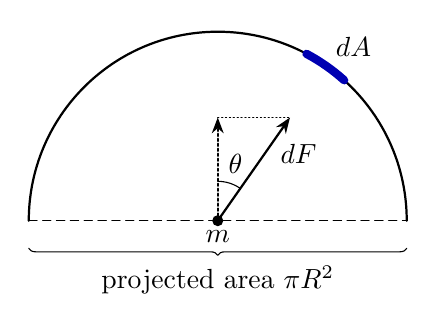
\begin{tikzpicture}[scale=1.0, line cap=round, line join=round, >={Stealth[length=2mm]}]
  \draw[thick] (2.4,0) arc[start angle=0, end angle=180, radius=2.4];
  \draw[densely dashed] (-2.4,0) -- (2.4,0);
  \fill (0,0) circle (2pt) node[below] {$m$};
  \coordinate (E) at (55:2.4);
  \draw[line width=3pt, blue!70!black] (48:2.4) arc[start angle=48, end angle=62, radius=2.4];
  \node[above right] at (E) {$dA$};
  \draw[->, thick] (0,0) -- (55:1.6) node[pos=0.65, right=2pt] {$dF$};
  \draw[->, thick, densely dotted] (0,0) -- (0,{1.6*sin(55)});
  \draw[densely dotted] (0,{1.6*sin(55)}) -- (55:1.6);
  \coordinate (Up) at (0,1);
  \coordinate (O) at (0,0);
  \pic[draw, "$\theta$", angle radius=5mm, angle eccentricity=1.5] {angle = E--O--Up};
  \draw[decorate, decoration={brace, mirror, raise=10pt}] (-2.4,0) -- (2.4,0) node[midway, below=13pt] {projected area $\pi R^2$};
\end{tikzpicture}
\end{center}

\section*{Problem 25}
You can do the full calculations, but it's best to approximate.
Write out the formula to understand the relationship between the quantities. $A=2\pi r\ell$, so $r$ and $\ell$ are multiplied, so we're dealing with relative (fractional) uncertainties.
For the radius, $\Delta r/r=0.1/1=10\%$, which is a lot compared to $\Delta\ell/\ell=0.01/1=1\%$.
No need to convert between cm and m, because relative uncertainties don't care about units; they cancel.
\begin{itemize}[leftmargin=*, itemsep=0.25em]
\item Method 1: upgrading the ruler addresses the 10\% error. It'll reduce to about 1\% because both $\Delta r/r$ and $\Delta\ell/\ell$ are now at 1\%.
\item Method 2: doesn't address the ruler. You can fix the 1\% error all you want, but the big problem remains. Still about 10\%.
\item Method 3: $\Delta_{\text{average}}=\Delta_{\text{one measurement}}/\sqrt N$. Initially we had about 10\%; divide by $\sqrt{10}$ to get about 3\%.
\end{itemize}
Clearly, 2 is the greatest error and 1 is the least.

\end{document}
